\documentclass[12pt]{article}
\usepackage[utf8]{inputenc}
\usepackage[T1]{fontenc}
\usepackage[english]{babel}
\usepackage{amsmath, amssymb, amsthm}
\usepackage{geometry}
\usepackage{titling}
\usepackage{fancyhdr}
\usepackage{lipsum}
\usepackage{parskip}
\usepackage{forest}
\usepackage{tikz}
\usepackage{stmaryrd}
\usepackage{listings}
\usepackage{graphicx}
\usepackage{float}
\usepackage{alphalph}
\usepackage{cancel}
\usepackage{textgreek}
\usepackage{titlesec}
\usepackage{dsfont}
\usepackage{caption}
\usepackage{listings}

\geometry{top=4cm, bottom=4cm, left=4cm, right=4cm}
\pagestyle{fancy}
\fancyhf{}
\rhead{Pierre Pili $\cdot$ Marie Gardie $\cdot$ Isée Biglietti}
\lhead{Econometrics 3}
\cfoot{\thepage}
\setlength{\headheight}{14.49998pt}
\addtolength{\topmargin}{-2.49998pt}

\titleformat{\section}{\small\bfseries}{\thesection}{1em}{}
\renewcommand{\thesubsection}{\arabic{section}.\arabic{subsection}}
\renewcommand{\thesubsubsection}{\arabic{section}.\arabic{subsection}.\alph{subsubsection}}

\title{Problem Set 7}
\author{PILI Pierre $\cdot$ GARDIE Marie $\cdot$ BIGLIETTI Isée}
\date{\today}

% Redéfinir le format de numérotation des sous-sections
\titleformat{\subsection}
  {\normalfont\small\bfseries}{\alph{subsection})}{1em}{}
  
\begin{document}
\maketitle
\renewcommand{\thesubsection}{\alph{subsection}}

\subsection{Regress the variable $survived$ on $female$. Report and interpret the estimated (marginal) “effect” of being female.}

% Table created by stargazer v.5.2.3 by Marek Hlavac, Social Policy Institute. E-mail: marek.hlavac at gmail.com
% Date and time: Mer, avr 24, 2024 - 15:56:03
\begin{table}[!htbp] \centering 
  \caption{OLS} 
  \label{olsa} 
\begin{tabular}{@{\extracolsep{5pt}}lc} 
\\[-1.8ex]\hline 
\hline \\[-1.8ex] 
 & \multicolumn{1}{c}{\textit{Dependent variable:}} \\ 
\cline{2-2} 
\\[-1.8ex] & survived \\ 
\hline \\[-1.8ex] 
 female & 0.536$^{***}$ \\ 
  & (0.024) \\ 
  & \\ 
 Constant & 0.191$^{***}$ \\ 
  & (0.014) \\ 
  & \\ 
\hline \\[-1.8ex] 
Observations & 1,309 \\ 
R$^{2}$ & 0.280 \\ 
Adjusted R$^{2}$ & 0.279 \\ 
Residual Std. Error & 0.413 (df = 1307) \\ 
F Statistic & 507.059$^{***}$ (df = 1; 1307) \\ 
\hline 
\hline \\[-1.8ex] 
\textit{Note:}  & \multicolumn{1}{r}{$^{*}$p$<$0.1; $^{**}$p$<$0.05; $^{***}$p$<$0.01} \\ 
\end{tabular} 
\end{table} 

The dependent variable $survived$ is a binary variable. We are thus in the binary outcome framework. In this question we perform an OLS regression of the $survived$
variable on the $female$ variable. The average survival rate was $0.191$ (see Table \ref{olsa}) while a woman would survive with a probability $0.191 + 0.536 = 0.727$.
Being a female increases your probability of survival by $0.536$. As the $female$ variable is binary, those numbers can be interpreted as probabilities. The result is very significant, being a female on board dramatically increased your chances of survival.

\subsection{Construct a 95\% confidence interval for the estimated (marginal) effect.}
Using the robust estimated variance we find a confidence interval at the 95\% level for the estimated marignal effect equal to $[0.488, 0.585]$.

\subsection{Repeat (a) using the probit. What do you find ? Are you surprised ?}

% Table created by stargazer v.5.2.3 by Marek Hlavac, Social Policy Institute. E-mail: marek.hlavac at gmail.com
% Date and time: Mer, avr 24, 2024 - 15:56:03
\begin{table}[!htbp] \centering 
  \caption{Probit Regression} 
  \label{prbtc} 
\begin{tabular}{@{\extracolsep{5pt}}lc} 
\\[-1.8ex]\hline 
\hline \\[-1.8ex] 
 & \multicolumn{1}{c}{\textit{Dependent variable:}} \\ 
\cline{2-2} 
\\[-1.8ex] & survived \\ 
\hline \\[-1.8ex] 
 female & 1.479$^{***}$ \\ 
  & (0.080) \\ 
  & \\ 
 Constant & $-$0.874$^{***}$ \\ 
  & (0.050) \\ 
  & \\ 
\hline \\[-1.8ex] 
Observations & 1,309 \\ 
Log Likelihood & $-$684.052 \\ 
Akaike Inf. Crit. & 1,372.103 \\ 
\hline 
\hline \\[-1.8ex] 
\textit{Note:}  & \multicolumn{1}{r}{$^{*}$p$<$0.1; $^{**}$p$<$0.05; $^{***}$p$<$0.01} \\ 
\end{tabular} 
\end{table} 

We observe that the model now gives us a negative constant term. The coefficient of interest in the probit regression is $\beta = 1.479$ (see Table \ref{prbtc}) which means that the marginal effect is positive which was expected, this is not the marginal effect however. Using the margins package, we find a marginal effect of $0.434$. Those results do not seem very surprising, the average marginal effect is lower than the one OLS came up with however. 

\stepcounter{subsection}
\subsection{Continuing with the probit model from (c), add a numeric copy of the variable pclass to the “regression”. Interpret your results.}
As in the previous question, we find a significant positive impact of being a female on board, with a significant negative impact of the new $pclass$ variable (see Table \ref{prbte}). Using the library margins, we find a marginal effect of $0.406$ for the female variable and $-0.133$ for the $pclass$ variable. The intuition is clear, the $pclass$ goes from $1$ to $3$ from the most expensive seat to the cheapest. Being in first class increased your chances of surival by a significant amount, but still less than being a female. Leonardo Dicaprio increased both coefficients in absolute value even though their was enough space on this little piece of wood...

% Table created by stargazer v.5.2.3 by Marek Hlavac, Social Policy Institute. E-mail: marek.hlavac at gmail.com
% Date and time: Mer, avr 24, 2024 - 15:56:04
\begin{table}[!htbp] \centering 
  \caption{Probit Regression} 
  \label{prbte} 
\begin{tabular}{@{\extracolsep{5pt}}lc} 
\\[-1.8ex]\hline 
\hline \\[-1.8ex] 
 & \multicolumn{1}{c}{\textit{Dependent variable:}} \\ 
\cline{2-2} 
\\[-1.8ex] & survived \\ 
\hline \\[-1.8ex] 
 female & 1.503$^{***}$ \\ 
  & (0.083) \\ 
  & \\ 
 pclass & $-$0.494$^{***}$ \\ 
  & (0.048) \\ 
  & \\ 
 Constant & 0.245$^{**}$ \\ 
  & (0.117) \\ 
  & \\ 
\hline \\[-1.8ex] 
Observations & 1,309 \\ 
Log Likelihood & $-$629.609 \\ 
Akaike Inf. Crit. & 1,265.218 \\ 
\hline 
\hline \\[-1.8ex] 
\textit{Note:}  & \multicolumn{1}{r}{$^{*}$p$<$0.1; $^{**}$p$<$0.05; $^{***}$p$<$0.01} \\ 
\end{tabular} 
\end{table} 


\subsection{Instead of adding a numeric copy of the variable pclass to the regression in (c), add the variable pclass to it (pclass is coded as a “factor”). Interpret your results.}
This time the models estimates two coefficients for two dummy variables, $pclass2$ which is equal to $1$ when the passager is in second class, and similarly for $pclass3$. This regression adds information to the previous one as only one coefficient was used to describe an incrementation in the pclass variable. Results are displayed in Table \ref{prbtf}. We see that, as expected, the cheaper the seat you bought, the less chances of survival you had. Using the library margins, I find a marginal effect of $0.406$ for the female variable, as before, $-0.169$ for the $pclass2$ variable and $-0.295$ for the $pclass3$ variable. It means that the impact from moving from first class to the third is about twice as bad as moving from first class to the second. Put otherwise, the effect of a one unit incrementation of the pclass variable seems constant.

% Table created by stargazer v.5.2.3 by Marek Hlavac, Social Policy Institute. E-mail: marek.hlavac at gmail.com
% Date and time: Mar, avr 23, 2024 - 11:49:31
\begin{table}[!htbp] \centering 
  \caption{Probit Regression} 
  \label{prbtf} 
\begin{tabular}{@{\extracolsep{5pt}}lc} 
\\[-1.8ex]\hline 
\hline \\[-1.8ex] 
 & \multicolumn{1}{c}{\textit{Dependent variable:}} \\ 
\cline{2-2} 
\\[-1.8ex] & survived \\ 
\hline \\[-1.8ex] 
 female & 1.503$^{***}$ \\ 
  & (0.083) \\ 
  & \\ 
 pclass2 & $-$0.537$^{***}$ \\ 
  & (0.115) \\ 
  & \\ 
 pclass3 & $-$0.994$^{***}$ \\ 
  & (0.097) \\ 
  & \\ 
 Constant & $-$0.236$^{***}$ \\ 
  & (0.083) \\ 
  & \\ 
\hline \\[-1.8ex] 
Observations & 1,309 \\ 
Log Likelihood & $-$629.527 \\ 
Akaike Inf. Crit. & 1,267.055 \\ 
\hline 
\hline \\[-1.8ex] 
\textit{Note:}  & \multicolumn{1}{r}{$^{*}$p$<$0.1; $^{**}$p$<$0.05; $^{***}$p$<$0.01} \\ 
\end{tabular} 
\end{table} 


\subsection{The model in (e) constitutes a restricted version of the model in (f). What is the restriction? Test it using a LR test. What do you find?}
The model estimated in question (f) writes
$$\mathbb{P}(survived = 1) = \phi(\alpha + \beta_1 female + \beta_2 pclass2 + \beta_3 pclass 3)$$
while the model the model in question (e) imposes the restriction $\beta_3 = 2 \beta_2$.
Performing the LR test using the lrtest function from the lmtest package, we find that the number of interest is 0.16 derived from a $\chi^2(1)$ distribution under the null. This value is below the rejection threshold at the 10 \% level, we cannot reject the null hypothesis.

\stepcounter{subsection}
\subsection{Starting with your model specification in (e), add the variable $fare$. Use the Wald test and the LR test to test whether the coefficient on $fare$ is equal to zero. What do you find?}

% Table created by stargazer v.5.2.3 by Marek Hlavac, Social Policy Institute. E-mail: marek.hlavac at gmail.com
% Date and time: Mer, avr 24, 2024 - 15:56:05
\begin{table}[!htbp] \centering 
  \caption{Probit Regression} 
  \label{prbti} 
\begin{tabular}{@{\extracolsep{5pt}}lc} 
\\[-1.8ex]\hline 
\hline \\[-1.8ex] 
 & \multicolumn{1}{c}{\textit{Dependent variable:}} \\ 
\cline{2-2} 
\\[-1.8ex] & survived \\ 
\hline \\[-1.8ex] 
 female & 1.494$^{***}$ \\ 
  & (0.084) \\ 
  & \\ 
 pclass & $-$0.470$^{***}$ \\ 
  & (0.057) \\ 
  & \\ 
 fare & 0.001 \\ 
  & (0.001) \\ 
  & \\ 
 Constant & 0.169 \\ 
  & (0.152) \\ 
  & \\ 
\hline \\[-1.8ex] 
Observations & 1,308 \\ 
Log Likelihood & $-$629.200 \\ 
Akaike Inf. Crit. & 1,266.399 \\ 
\hline 
\hline \\[-1.8ex] 
\textit{Note:}  & \multicolumn{1}{r}{$^{*}$p$<$0.1; $^{**}$p$<$0.05; $^{***}$p$<$0.01} \\ 
\end{tabular} 
\end{table} 

The LR does not reject the null as the outcome of the $\chi^2(1)$ distribution is $0.59$ and is below the rejection threshold at the 10 \% level meaning that the $fare$ coefficient is not statstically different from 0. We see in Table \ref{prbti} that the coefficient is not significant at the 10 \% level according to the Wald test automatically performed. Both tests fail to reject the null. The variable $fare$ does not seem to have any impact on the survival rate on board.

\subsection{Starting with your model specification in (e), add the variable age. Compute the partial effect of age for a female passenger in 1st class with “average” age.}

% Table created by stargazer v.5.2.3 by Marek Hlavac, Social Policy Institute. E-mail: marek.hlavac at gmail.com
% Date and time: Mer, avr 24, 2024 - 15:56:06
\begin{table}[!htbp] \centering 
  \caption{Probit Regression} 
  \label{prbtj} 
\begin{tabular}{@{\extracolsep{5pt}}lc} 
\\[-1.8ex]\hline 
\hline \\[-1.8ex] 
 & \multicolumn{1}{c}{\textit{Dependent variable:}} \\ 
\cline{2-2} 
\\[-1.8ex] & survived \\ 
\hline \\[-1.8ex] 
 female & 1.484$^{***}$ \\ 
  & (0.094) \\ 
  & \\ 
 pclass & $-$0.641$^{***}$ \\ 
  & (0.062) \\ 
  & \\ 
 age & $-$0.019$^{***}$ \\ 
  & (0.004) \\ 
  & \\ 
 Constant & 1.160$^{***}$ \\ 
  & (0.215) \\ 
  & \\ 
\hline \\[-1.8ex] 
Observations & 1,046 \\ 
Log Likelihood & $-$492.797 \\ 
Akaike Inf. Crit. & 993.594 \\ 
\hline 
\hline \\[-1.8ex] 
\textit{Note:}  & \multicolumn{1}{r}{$^{*}$p$<$0.1; $^{**}$p$<$0.05; $^{***}$p$<$0.01} \\ 
\end{tabular} 
\end{table} 

Denoting $\bar{age}$ as the mean age of the population and denoting the model
$$\mathbb{P}(survived = 1) = \phi(\alpha + \beta_1 female + \beta_2 pclass + \beta_3 age),$$ the partial marginal impact of age 
the partial marginal impact of interest is given by $\beta_3 \phi(\alpha + \beta_1 + \beta_2 + \beta_3 \bar{age})$ and we find $-0.0176$.

\subsection{Using your model specification in (j), compute the average partial effect of age. What do you find?}
Computing the average marginal effect using the predicition package, I find $-0.007$.

\subsection{Using your model specification in (j), plot the sorted marginal effect of age. What do you find ?}
\begin{figure}[ht]
    \centering
    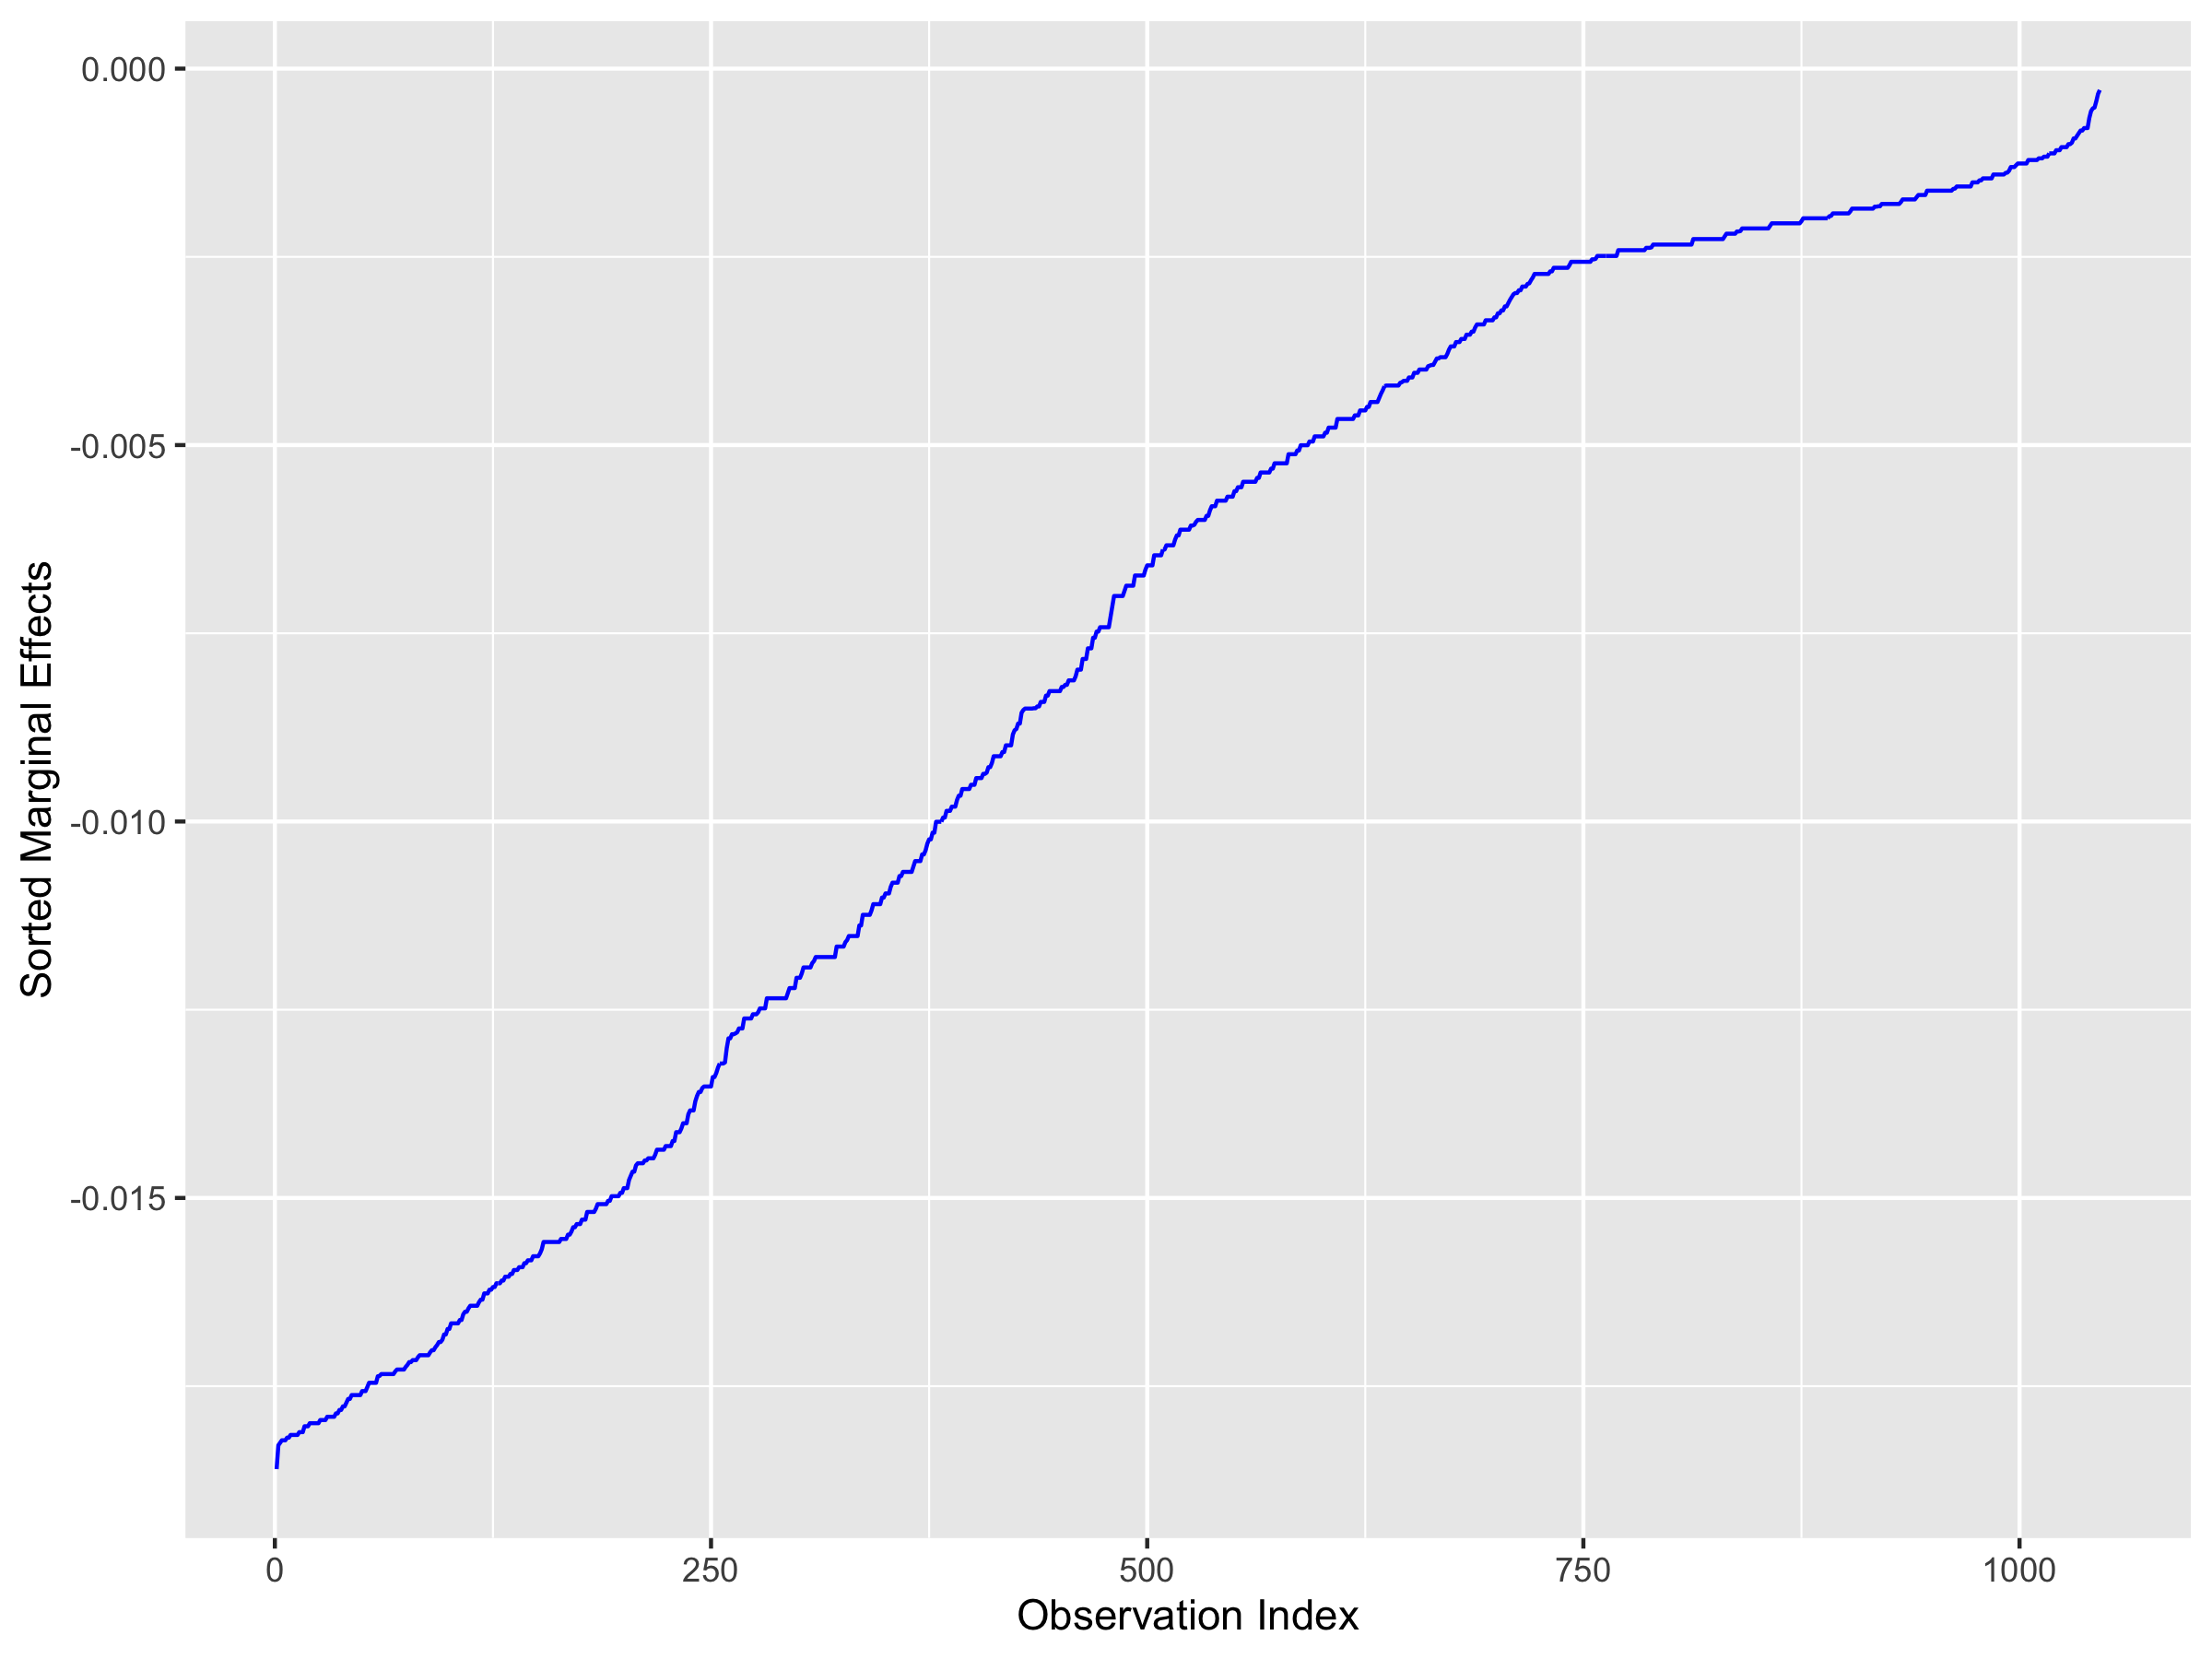
\includegraphics[width=0.8\textwidth]{OUTPUT/sorted_marginal_effects.png}
    \caption{Sorted Marginal Effect}
    \label{fig:sorted_marginal_effect}
  \end{figure}

  \begin{figure}[ht]
    \centering
    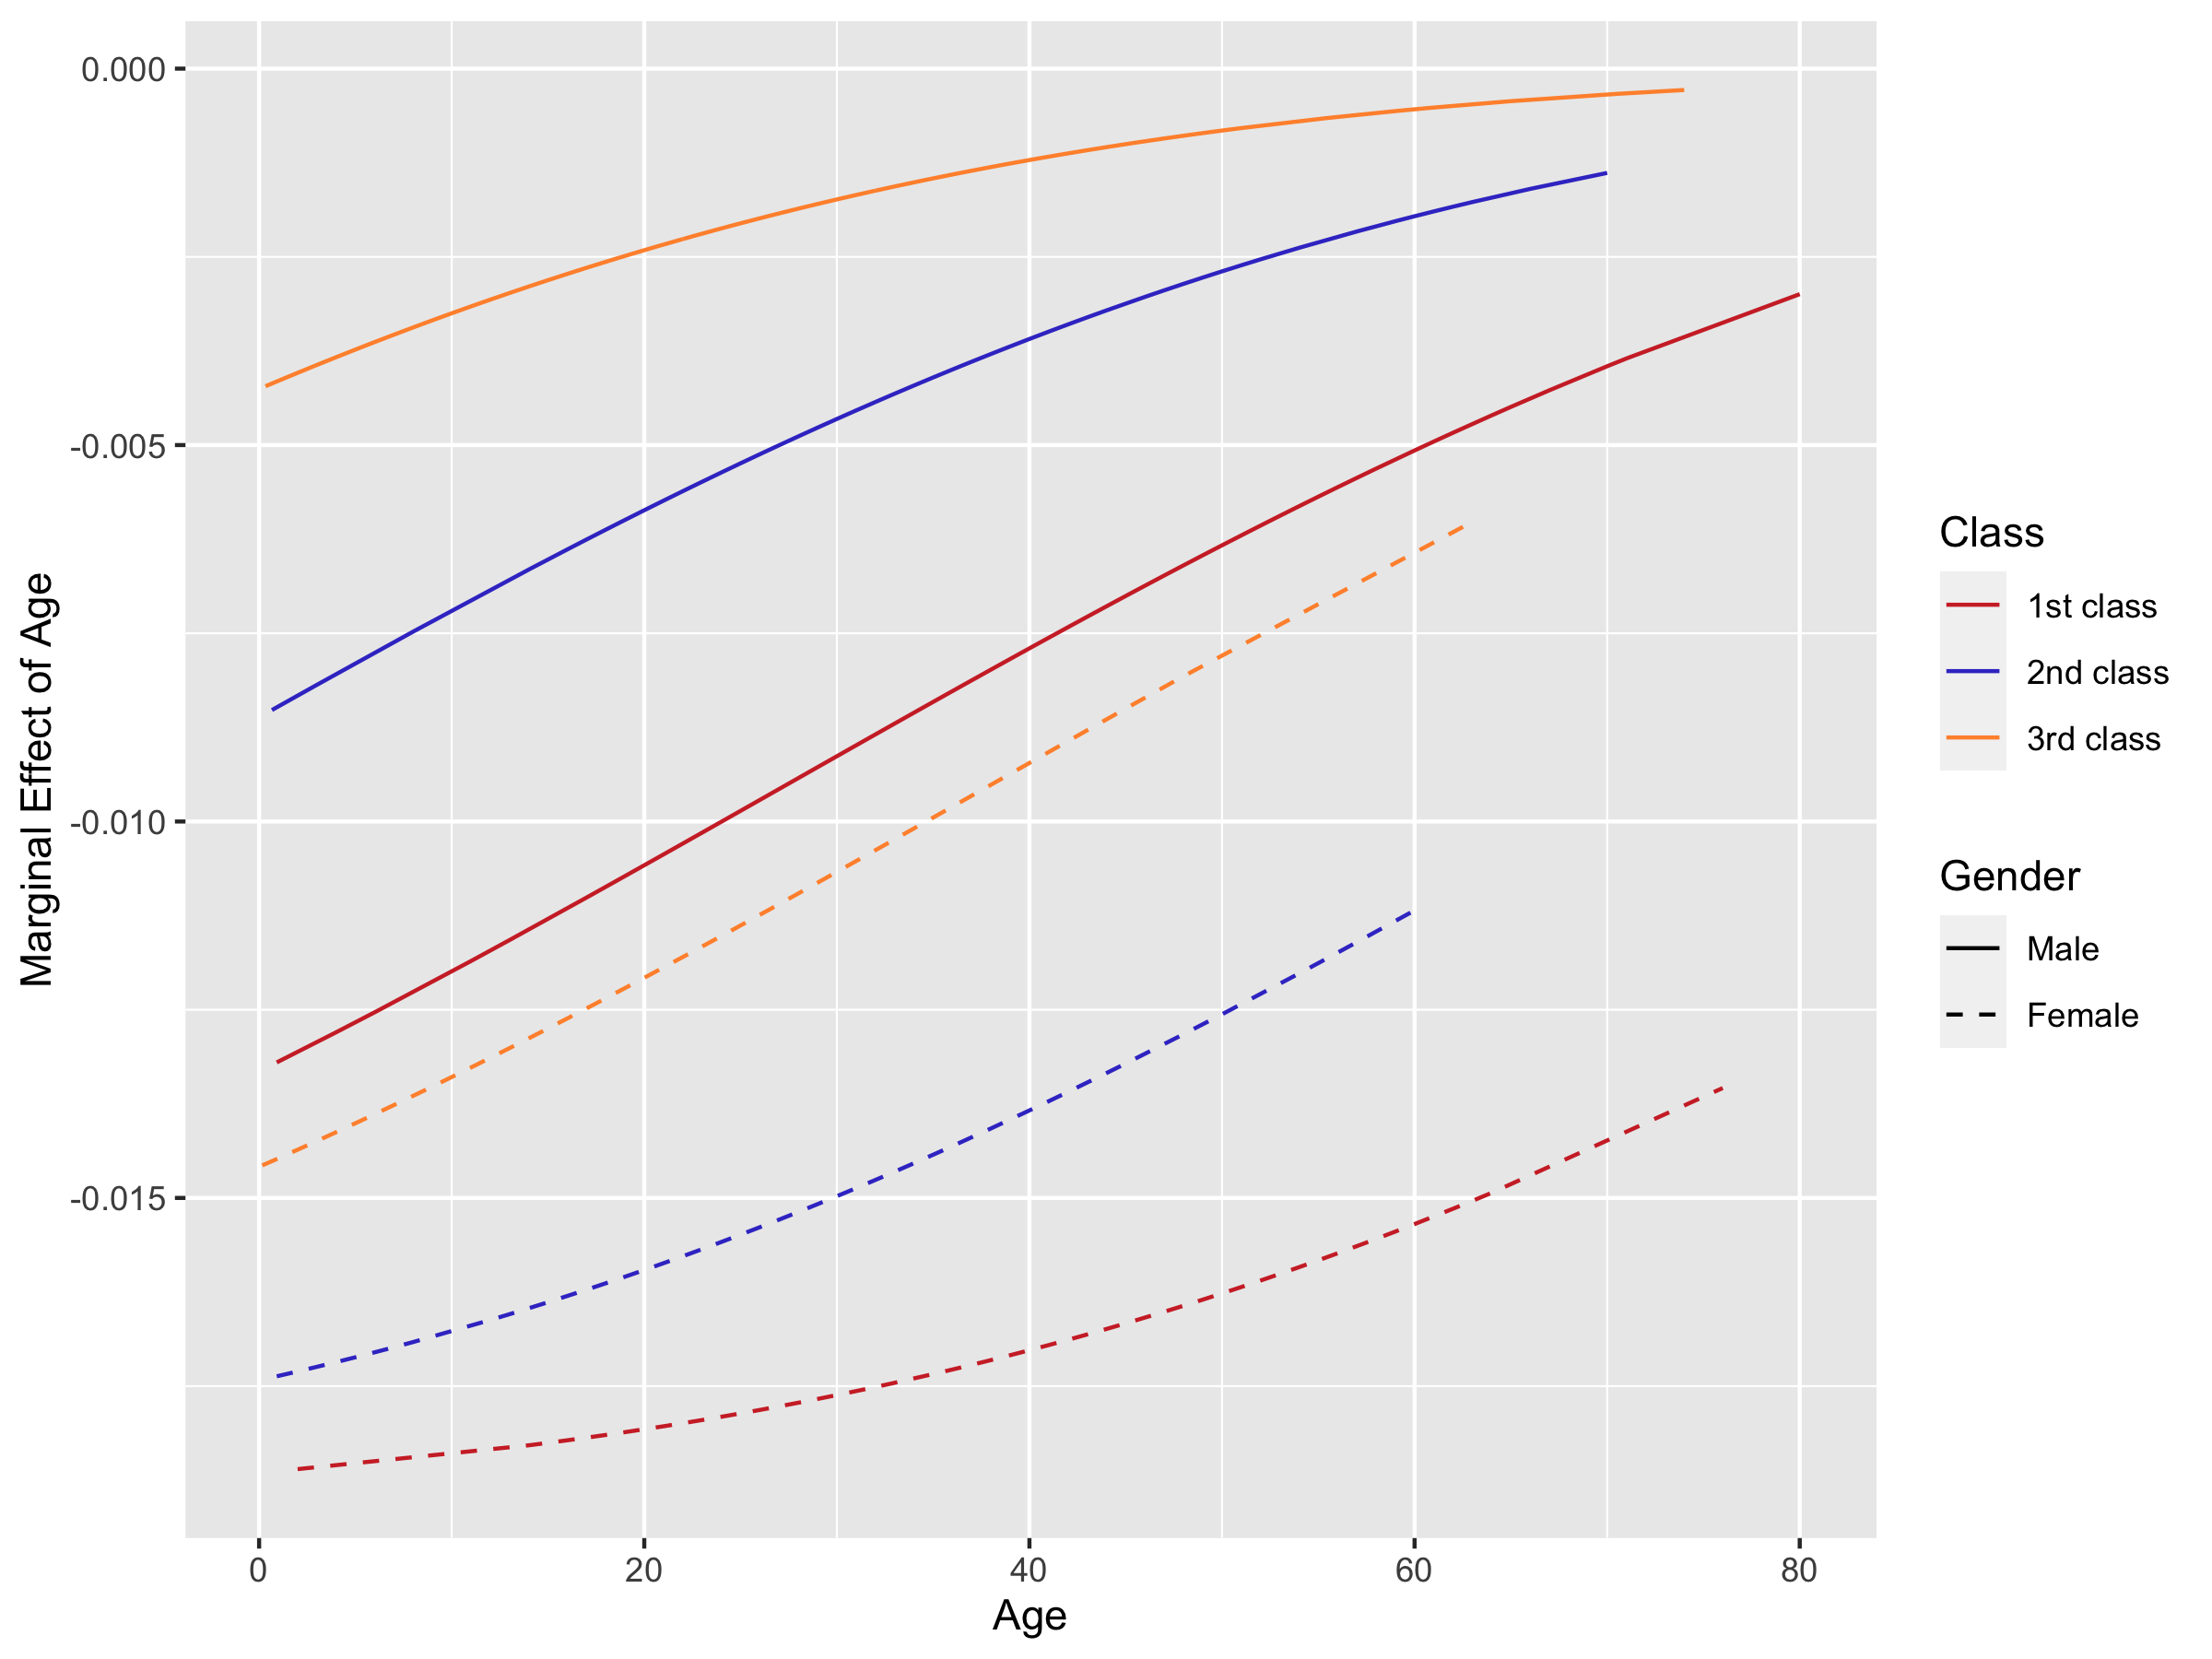
\includegraphics[width=0.8\textwidth]{OUTPUT/marginal_effect_age.png}
    \caption{Marginal effect of Age per Class and Gender}
    \label{fig:marginal_effect_age}
  \end{figure}
In figure \ref{fig:sorted_marginal_effect}, we find that the marginal is not constant and varies from $0$ to $0.015$ in absolute value. Plotting the marginal effect with respect to $age$ for each subgroup of people (see figure \ref{fig:marginal_effect_age}) shows that the marginal effect of the age on the survival rate is descreasing in absolute value with respect to age after controlling for gender and $pclass$.
\end{document}



